\chapter{基于生成对抗网络的多目标形变图像翻译}

\section{引言}

图像翻译旨在学习从一个图像域到另一个图像域的映射,可广泛应用于图像着色、超分辨率和风格迁移等任务中,非配对图像翻译如CycleGAN\cite{zhu2017unpaired}和DiscoGAN\cite{kim2017learning}等可以通过使用生成对抗网络进行深度学习,使用循环一致性损失来解决缺少配对数据集的问题,能够在马和斑马、苹果和橘子等数据集上取得较好的效果,实现在图像域之间传递复杂的局部纹理外观。图\ref{fig:cyclegan_failure}展示了CycleGAN无法实现狗转猫或者猫转狗的翻译,这是因为猫和狗两个域之间不仅存在纹理上的差异,还存在形状上的不同,这对之前的图像翻译方法来说具有挑战性。

\begin{figure}[ht]
    \centering
	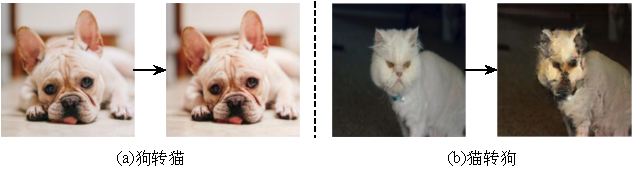
\includegraphics[width=\textwidth]{figs/cyclegan_failure.pdf}
	\caption{CycleGAN在有较大形状差异数据集上的翻译结果。图片来自文献\cite{zhu2017unpaired}。}
	\label{fig:cyclegan_failure}
\end{figure}

当图像中仅存在一个需要做形变翻译的目标,我们称此类任务为单目标形变图像翻译,近年来一些工作如U$-$GAT$-$IT\cite{kim2019u}、TransGaGa\cite{wu2019transgaga}等聚焦于单目标形变图像翻译,利用注意力机制或几何信息等方式取得令人满意的结果。但很多时候,图像中的目标并非一个,而是多个目标同时存在,如野外环境中多只羊翻译为多只长颈鹿,本节的工作即做此任务,称为多目标形变图像翻译,在实现形变的同时思考如何处理多个目标的图像翻译。为了解决此问题,我们将形状、纹理和背景分开处理,并利用第二节提到的循环一致性思想,提出一个基于生成对抗网络的模型,最终实现具有较大形状变化的多目标图像翻译,从而可以将图像翻译的实用性提高到一个新的水平。

\section{模型算法}

多目标形变图像翻译需要考虑的问题有两个:(1)如何确定每个目标;(2)如何实现形变。受InstaGAN\cite{mo2018instagan}启发,我们利用实例分割图确定每个目标的位置和形状,获得多个目标的实例信息。在探索过程中发现(如图\ref{fig:mask}),对于同样的网络,当在两个图像域之间翻译时,难以实现形状变化,但当在两个实例分割域之间做翻译时,可以实现形状的变化,因此我们提出将背景、形状和纹理分开处理。利用实例分割图实现两个域中多个目标在形状上的翻译,然后学习图像域的纹理特征,向翻译后的形状增添纹理信息,得到完整的翻译后的前景目标,再将此前景目标与背景结合,并经过一个细化网络,最终实现多目标形变图像翻译。

\begin{figure}[ht]
    \centering
	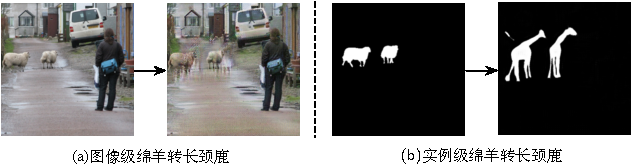
\includegraphics[width=\textwidth]{figs/mask.pdf}
	\caption{图像级和实例级的绵羊转长颈鹿结果。}
	\label{fig:mask}
\end{figure}

\subsection{算法框架}

给定两个图像域$X$和$Y$,并规定其对应的实例域为$M_X$和$M_Y$,对于图像$x\in X$和其对应的实例分割图$m_x\in M_X$,我们的任务是在保持其背景不变的情况下,将目标的形状和纹理翻译至$Y$域。我们将此问题分为四个部分:形状翻译、纹理翻译、背景翻译和进一步处理融合图像的细化网络,下面将详细介绍。

\begin{figure}[ht]
    \centering
	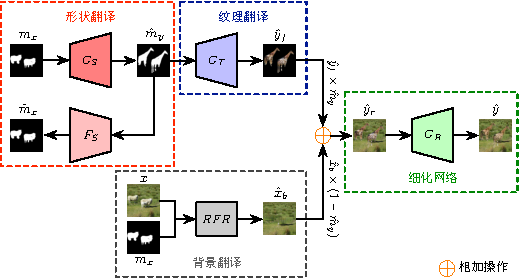
\includegraphics[width=\textwidth]{figs/multi_instance.pdf}
	\caption{多目标形变图像翻译模型示意图。}
	\label{fig:multi_instance}
\end{figure}

\subsubsection{形状翻译}

如图\ref{fig:multi_instance}中红色虚线框部分所示,我们在两个实例分割域之间进行翻译,因训练所用的数据集不配对,所以我们采用循环一致\cite{zhu2017unpaired}的训练方式。给定两个域$M_X$和$M_Y$,我们的目标是学习两个域之间的映射:$G_S: M_X\to M_Y$和$F_S: M_Y\to M_X$,实例分割图$m_x\in M_X$经生成器$G_S$合成$\hat{m}_y=G_S(m_x)$,并利用判别器$D_{S_y}$区分$\hat{m}_y$和$m_y\in M_Y$,然后利用生成器$F_S$将$\hat{m}_y$翻译为重建图像$\tilde{m}_x$,并约束$F_S(G_S(m_x))\approx m_x$使重建图像与输入图像接近。

\subsubsection{纹理翻译}

给定经过形状翻译的实例分割图$\hat{m}_y$,在纹理翻译部分的目的是向$\hat{m}_y$上添加属于$Y$域的纹理(如图\ref{fig:multi_instance}中蓝色虚线框部分所示),它要求网络可以准确定位到需要添加纹理的位置并学习需添加的纹理样式。类似于文献\cite{yang2019controllable},我们将此问题看作:给定配对数据\{$m_y$, $y$\},其中$y$为来自Y域的图像,$m_y\in M_Y$是与$y$相对应的实例分割图,训练一个纹理生成器$G_T$,使之可以学习映射$G_T: M_Y\to Y$。需要提到的一点是,因为我们希望网络仅学习实例分割图中标注的部分,因此为了更精准地训练和学习,排除其它位置的信息对纹理生成器的影响,我们仅取出$y$中与$m_y$相对应的部分(记作$y_f$)看作真实图像,因此判别器$D_T$对生成图像$\hat{y}_f=G_T(\hat{m}_y)$和真实图像$y_f$进行判别。

\subsubsection{背景翻译}

因为做图像翻译的两个域在形状上相差较大,如果直接用生成的目标替代原本的目标,那么在生成图像中很容易出现生成目标的周围还残留部分原目标内容的情况,使整个图像看起来不和谐。得益于图像修复的发展,我们利用一个图像修复算法RFR\cite{li2020recurrent}将图像$x$中与$m_x$相对应的部分进行修复,得到一个相对完整的背景$\hat{x}_b$。

\subsubsection{细化网络}

经过前面三个部分的训练,我们现在可以得到经过形状翻译的实例分割图$\hat{m}_y$、经过纹理翻译的前景目标$\hat{y}_f$和经过背景翻译的背景$\hat{x}_b$,利用公式\ref{eq:refine}将这三部分融合到一张图像中,即图\ref{fig:multi_instance}绿色虚线框部分中的$\hat{y}_r$,此时的融合图像存在前景目标与背景之间衔接不自然以及纹理部分生成粗糙等问题,为了解决这些问题,我们引入一个细化生成器$G_R$,得到最终的生成图像$\hat{y}=G_R(\hat{y}_r)$。
\begin{equation}
\begin{split}
\hat{y}_r=\hat{y}_f\times\hat{m}_y+\hat{x}_b\times(1-\hat{m}_y)
\end{split}
\label{eq:refine}
\end{equation}

\subsection{目标函数}

\subsubsection{形状翻译}

我们的目标函数有两项:用于将生成图像的分布尽量逼近目标域中的数据分布的对抗损失\cite{goodfellow2014generative}和防止学习到的映射$G_S$与$F_S$相矛盾的循环一致性损失\cite{zhu2017unpaired}。对于映射$G_S: M_X\to M_Y$和相应的判别器$D_{S_y}$,我们定义对抗损失为:
\begin{equation}
\begin{split}
\mathcal{L}_{adv\_x}^{shape}=\mathbb{E}_{m_y}[\log D_{S_y}(m_y)] + \mathbb{E}_{m_x}[\log(1-D_{s_y}(G_S(m_x))]
\end{split}
\label{eq:shape_x}
\end{equation}
其中生成器$G_S$的目的在于使生成的图像看起来属于$M_Y$域,而判别器$D_{S_y}$旨在分辨出生成器合成的图像$\hat{m_y}$和真实图像$m_y$。对于映射$F_S: M_Y\to M_X$和判别器$D_{S_x}$,我们定义此方向的对抗损失为:
\begin{equation}
\begin{split}
\mathcal{L}_{adv\_y}^{shape}=\mathbb{E}_{m_x}[\log D_{S_x}(m_x)] + \mathbb{E}_{m_y}[\log(1-D_{s_x}(F_S(m_y))]
\end{split}
\label{eq:shape_y}
\end{equation}
其中生成器$F_S$和判别器$D_{S_x}$的目的分别与$G_S$和$D_{S_y}$类似。将两个方向的对抗损失合并,得完整的对抗损失:
\begin{equation}
\begin{split}
\mathcal{L}_{adv}^{shape}=\mathcal{L}_{adv\_x}^{shape}+\mathcal{L}_{adv\_y}^{shape}。
\end{split}
\label{eq:shape_adv}
\end{equation}

为了进一步减少可能的映射函数的空间,解决无配对训练数据的弊端,我们还加入循环一致性损失,对于来自$M_X$域的图像$m_x$,经过一个循环,应可以重建回原始图像,即$F_S(G_S(m_x))\approx m_x$,类似地,对来自$M_Y$中的图像$m_y$,也应满足$G_S(F_S(m_y))\approx m_y$,损失函数定义为:
\begin{equation}
\begin{split}
\mathcal{L}_{cyc}^{shape}=\mathbb{E}_{m_x}[\parallel F_S(G_S(m_x))-m_x\parallel_1]+\mathbb{E}_{m_y}[\parallel G_S(F_S(m_y))-m_y\parallel_1]。
\end{split}
\label{eq:shape_cyc}
\end{equation}
综合公式\ref{eq:shape_adv}和公式\ref{eq:shape_cyc},可得形状翻译部分的总损失函数:
\begin{equation}
\begin{split}
\min \limits_{G_S, F_S} \max \limits_{D_{S_x}, D_{S_y}} \mathcal{L}_{total}^{shape}=\lambda_{adv}^{shape}\mathcal{L}_{adv}^{shape}+\lambda_{cyc}^{shape}\mathcal{L}_{cyc}^{shape}
\end{split}
\label{eq:shape}
\end{equation}
其中$\lambda_{adv}^{shape}$和$\lambda_{cyc}^{shape}$为平衡不同损失贡献度的超参数。

\subsubsection{纹理翻译}

我们的目标函数包括条件对抗损失、重建损失和颜色损失,条件对抗损失可以使生成的图像$\hat{y}_f$符合真实前景图像$y_f$所属于的$Y_F$域的分布,定义为:
\begin{equation}
\begin{split}
\mathcal{L}_{adv}^{texture}=\mathbb{E}_{m_y,y_f}[\log D_T(m_y,y_f)]+\mathbb{E}_{m_y,y_f}[\log(1-D_T(m_y,G_T(m_y)))]
\end{split}
\label{eq:texture_adv}
\end{equation}

之前的研究发现,将对抗损失与传统的非结构化回归损失相结合,可以生成更逼真的样本,如L2\cite{pathak2016context}和L1损失\cite{isola2017image}\cite{shrivastava2017learning},考虑到L1损失可以使生成样本产生较少的模糊,因此引入L1损失,定义为:
\begin{equation}
\begin{split}
\mathcal{L}_{rec}^{texture}=\mathbb{E}_{m_y,y_f}[\parallel G_T(m_y)-y_f\parallel_1]
\end{split}
\label{eq:texture_rec}
\end{equation}

因为L1损失仅在数值上度量色差,不能保证颜色向量具有相同的方向,因此用L1损失可能导致明显的颜色不匹配,在此我们引入颜色损失\cite{wang2019underexposed}以保证生成的纹理与真实纹理之间的颜色尽量一致,颜色损失具体定义为:
\begin{equation}
\begin{split}
\mathcal{L}_{col}^{texture}=\sum_{p}\angle((G_T(m_y)_p),(y_f)_p)
\end{split}
\label{eq:texture_col}
\end{equation}
其中$()_p$代表一个像素,$\angle(,)$是将RGB颜色作为3D矢量计算两种颜色之间角度的运算符。

综合以上三个公式,可定义纹理翻译部分的总目标函数为:
\begin{equation}
\begin{split}
\min \limits_{G_T} \max \limits_{D_T} \mathcal{L}_{total}^{texture}=\lambda_{adv}^{texture}\mathcal{L}_{adv}^{texture}+\lambda_{rec}^{texture}\mathcal{L}_{rec}^{texture}+\lambda_{col}^{texture}\mathcal{L}_{col}^{texture}
\end{split}
\label{eq:texture}
\end{equation}
其中$\lambda_{adv}^{texture}$、$\lambda_{rec}^{texture}$和$\lambda_{col}^{texture}$为平衡$\mathcal{L}_{adv}^{texture}$、$\mathcal{L}_{rec}^{texture}$和$\mathcal{L}_{col}^{texture}$的超参数。

\subsubsection{细化网络}

对于细化网络,我们希望生成的图像符合$Y$域的真实样本的分布,但又保证其背景与原图像一致。对于背景区域,我们引入L1损失使生成图像$\hat{y}=G_R(\hat{y}_r)$的背景与融合图像$\hat{y}_r$的背景保持一致,损失函数定义为:
\begin{equation}
\begin{split}
\mathcal{L}_{rec}^{refine}=\mathbb{E}_{\hat{y}_r, \hat{y}}[\parallel \hat{y}\times(1-\hat{m}_y)-\hat{y}_r\times(1-\hat{m}_y)\parallel_1]
\end{split}
\label{eq:refine_rec}
\end{equation}

受图像风格迁移算法的影响,图像翻译领域也引入一种思想:使用预先训练的网络分别提取生成图像和真实图像的特征,通过比较特征使生成图像与真实图像在语义上更加相似,即感知损失\cite{johnson2016perceptual},我们利用感知损失限制生成图像的前景与真实图像的前景之间的差异:
\begin{equation}
\begin{split}
\mathcal{L}_{per}^{refine}=\mathbb{E}_{y}\sum_{i=1}^{T}\frac{1}{N_i}[\parallel\Phi_{VGG}^i(\hat{y}\times\hat{m}_y)-\Phi_{VGG}^i(y\times\hat{m}_y)\parallel_1]
\end{split}
\label{eq:refine_per}
\end{equation}
其中$T$代表总层数,$N_i$代表每一层元素的数量,$\Phi_{VGG}^i$代表VGG网络的第$i$层特征图。

除此之外,我们还加入对抗损失函数来约束生成图像的分布,使之与$Y$域的分布相匹配,优化生成图像的质量,损失函数定义为:
\begin{equation}
\begin{split}
\mathcal{L}_{adv}^{refine}=\mathbb{E}_y[\log D_R(y)] + \mathbb{E}_y[\log(1-D_R(\hat{y}))] 
\end{split}
\label{eq:refine_adv}
\end{equation}

综上,我们将公式\ref{eq:refine_rec}、\ref{eq:refine_per}和\ref{eq:refine_adv}线性加权组合,得到细化网络部分最终的目标函数:
\begin{equation}
\begin{split}
\min \limits_{G_R} \max \limits_{D_R} \mathcal{L}_{total}^{refine}=\lambda_{rec}^{refine}\mathcal{L}_{rec}^{refine}+\lambda_{per}^{refine}\mathcal{L}_{per}^{refine}+\lambda_{adv}^{refine}\mathcal{L}_{adv}^{refine}
\end{split}
\label{eq:refine_total}
\end{equation}
其中$\lambda_{rec}^{refine}$、$\lambda_{per}^{refine}$和$\lambda_{adv}^{refine}$是超参数,用于控制目标函数中各项对总损失的贡献程度。

\subsection{模型部署}

\textbf{网络架构}~形状生成器、纹理生成器和细化生成器都由卷积神经网络层构成,下采样阶段使用卷积层、$ReLU$激活函数和实例正则化,中间阶段使用残差块,上采样阶段采用反卷积层、$ReLU$激活函数和实例正则化的组合,不同的是纹理生成器引入跳连接\cite{ronneberger2015u},将下采样和上采样过程中分辨率相同的特征图按通道拼接,使输入和输出之间存在的大量低层信息直接在网络上传递,所有信息流通过所有的层,从而提升纹理生成的效果。形状判别器采用多尺度判别器\cite{wang2018high},以用于更好地学习具有形变的图像翻译任务,且每一层都引入光谱正则化以稳定训练。

\textbf{训练细节}~对于所有的实验,我们设置超参数$\lambda_{adv}^{shape}$=$\lambda_{adv}^{texture}$=1,$\lambda_{adv}^{refine}=0.1$,$\lambda_{cyc}^{shape}$=$\mathcal{L}_{col}^{texture}$=$\lambda_{rec}^{refine}$=$\lambda_{per}^{refine}$=10,$\lambda_{rec}^{texture}$=100。

\section{实验}

\subsection{数据集设置}

\textbf{绵羊}$\leftrightarrow$\textbf{长颈鹿}~图像(如图\ref{fig:shp2gir_coco})来自于COCO数据集\cite{lin2014microsoft},其中绵羊域包含1516张训练图像和实例分割图,长颈鹿域包含2536张训练图像和实例分割图,数据集中的图像裁剪为256$\times$256分辨率。测试集包括64张绵羊图像和101张长颈鹿图像及其实例分割图。

\begin{figure}[ht]
    \centering
  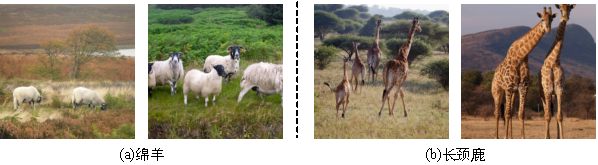
\includegraphics[width=\textwidth]{figs/shp2gir_coco.pdf}
  \caption{绵羊$\leftrightarrow$长颈鹿数据集示意图。图片来自文献\cite{lin2014microsoft}。}
  \label{fig:shp2gir_coco}
\end{figure}

\subsection{对比方法}

\textbf{CycleGAN}~作为非配对图像翻译的开山之作,Zhu等人\cite{zhu2017unpaired}提出的CycleGAN在多个数据集上取得令人信服的结果。

\textbf{U-GAT-IT}~Kim等人\cite{kim2019u}提出的U-GAT-IT引入一个注意力模块,通过基于辅助分类器得到的注意力图使模型更关注图像中可以区分两个域的区域,同时提出的自适应层实例归一化函数是利用在训练过程中从数据集中学到的参数在层归一化和实例归一化之间选择合适的比率。U-GAT-IT可以通过注意力机制和可学习的归一化函数使网络能够翻译需要整体变化或有较大形状变化的图像,因此与其对比。

\textbf{GANHopper}~Lira等人\cite{lira2020ganhopper}提出的GANHopper通过多个跳在两个域之间逐步翻译图像,网络不直接执行翻译,而是通过要求网络生成中间图像来控制翻译,这些中间图像类似于来自输入域图像之间的加权混合,但不对中间图像进行训练,所有跳都是用一个生成器沿着每个方向产生的,除此之外,还添加了一个平滑项来约束每个跳的大小。GANHopper在有形变的数据集(如狗转猫、人脸转猫脸)中可以实现翻译。

\textbf{InstaGAN}~Mo等人\cite{mo2018instagan}提出的InstaGAN利用实例分割图将目标分离,使每个目标有属于自己的实例分割图,将图像输入到图像编码器,此图像中每个目标的实例分割图逐个输入到实例编码器中,将得到的图像特征图与实例特征图按通道拼接并分别进入图像解码器和实例解码器得到生成图像和生成的实例分割图,生成的图像可以实现多目标形变图像翻译。

\subsection{评价指标}

$\mathbf{FID}$~Fr$\mathrm{\acute{e}}$chet Inception Distance(FID\cite{heusel2017gans})作为对现有的Inception Score(IS\cite{salimans2016improved})的改进而被提出。IS应用了效果优异的图像分类网络Inception v3,此网络可以对一组图像做分类预测,IS基于分类情况计算分数,但IS存在一个问题:仅考虑了生成图像的清晰度和多样性,而忽略了真实数据的影响。生成对抗网络的初衷是希望生成图像的分布尽量接近真实图像的分布,很显然,IS不能满足这一条件,因此FID应运而生,它可以更好地反映生成图像相较于真实图像的逼真度。

类似于IS,FID也使用了Inception v3模型,不同的是,FID并没有用Inception v3模型中最后一个用于分类的全连接层,而是提取了全连接层之前的2048维向量,因此每个图像被预测为2048个特征,可视为一个向量。对于真实图像,这个2048维向量是服从一个分布的,对于生成的图像,由它预测得到的向量也是一个分布,GAN的目标是使这两个分布尽量相同,问题此时转化为如何计算两个分布之间的距离。计算两个分布之间的距离,数学上可用Fr$\mathrm{\acute{e}}$chet距离或Wasserstein-2距离计算。

一个高斯分布可通过均值和方差确定,反过来说,如果给定两个相同的均值和方差,那么由这两个均值和方差确定的两个高斯分布相同,因此可以利用均值和方差来计算两个高斯分布之间的距离,两个分布之间的距离被定义为Fr$\mathrm{\acute{e}}$chet Inception Distance,即FID评价指标,可用公式表示为:
\begin{equation}
\begin{split}
FID(x,g)=\parallel\mu_x-\mu_g\parallel_2^2+Tr(\varSigma_x+\varSigma_g-2(\varSigma_x\varSigma_g)^{\frac{1}{2}})
\end{split}
\label{eq:FID}
\end{equation}
其中,$x$和$g$分别代表真实图像和生成图像,$\mu_x$和$\mu_g$表示的各自特征向量的均值,$\varSigma_x$和$\varSigma_g$为各自特征向量的协方差矩阵,$Tr$代表矩阵的迹(主对角线各元素的和)。FID的分数越低,即生成图像与真实图像之间的距离越小,代表生成图像的质量越好。

$\mathbf{LPIPS}$~Learned Perceptual Image Patch Similarity (LPIPS\cite{zhang2018perceptual})可用于衡量配对图像之间的相似程度。传统的图像相似度评价指标侧重于结构、内容等方面,优点为计算简单,但存在一个明显的缺点:与人的视觉感知存在较大差异,LPIPS指标的一大特点就是其得到的结果和人的视觉评价有更高的相关性。

假定有两幅图像$x$和$x_0$,利用一个预训练网络得到它们的深层特征,并计算出其特征之间的距离,从而得到$x$和$x_0$之间的相似性。为了评价生成结果的多样性,我们将从生成结果中随机采样,组成$n\times10$个图像对,其中$n$为数据集中图像的数量,然后计算每对图像之间的相似性,并将最终的平均值作为评价翻译结果多样性的LPIPS指标,LPIPS指标越大,代表翻译结果的内部多样性越好,反之越差。

\subsection{实验结果与分析}

\subsubsection{主观定性评价}

我们在绵羊$\leftrightarrow$长颈鹿数据集中实现两个方向的翻译,图\ref{fig:shp2gir}显示了绵羊转长颈鹿的定性结果,可以看出CycleGAN虽然可以生成长颈鹿的纹理且实现颈部拉长的效果,但不能生成一个完整的长颈鹿。U-GAT-IT对单个且清晰的绵羊可以实现翻译,但当绵羊的数量增多时,翻译无法完成,且与其它方法对比,其背景改动
\begin{figure}[ht]
    \centering
  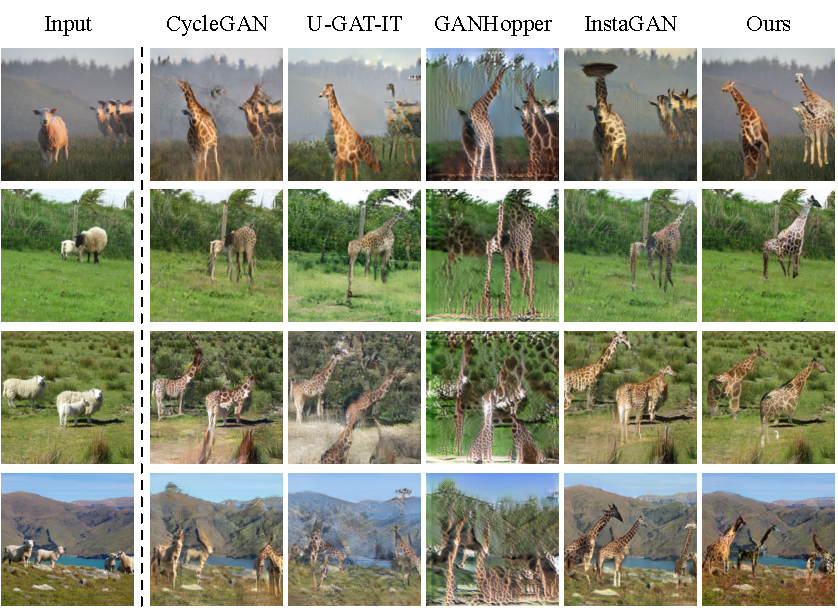
\includegraphics[width=\textwidth]{figs/shp2gir.pdf}
  \caption{绵羊转长颈鹿的定性结果图。}
  \label{fig:shp2gir}
\end{figure}
较大。GANHopper是这几种方法中效果最差的,整幅生成图像的目标和纹理都很混乱,InstaGAN可以部分实现绵羊至长颈鹿的翻译,但我们的方法相比较来说生成效果更好,多只绵羊都可以拥有长颈鹿的形状而不仅是纹理。


图\ref{fig:gir2shp}展示了长颈鹿转绵羊的定性结果,在此方向上的翻译效果整体比绵羊转长颈鹿的效果差一些,是因为数据集中大多数图像中的绵羊数量很多,目标物之间大多重叠且形态各异,给网络的学习增加了一定的难度。从图中可以看出,CycleGAN在形状上基本无变化,且纹理仍保留长颈鹿的纹理。U-GAT-IT的效果与CycleGAN类似,也无法实现翻译,但能看出其在形状上有一定的变化。GANHopper整体图像呈现模糊的效果,背景和前景目标都没有清楚的样式。InstaGAN和我们的方法在形状上都有变化,我们的方法可以实现每个目标都有更大程度的形变。

\begin{figure}[ht]
    \centering
  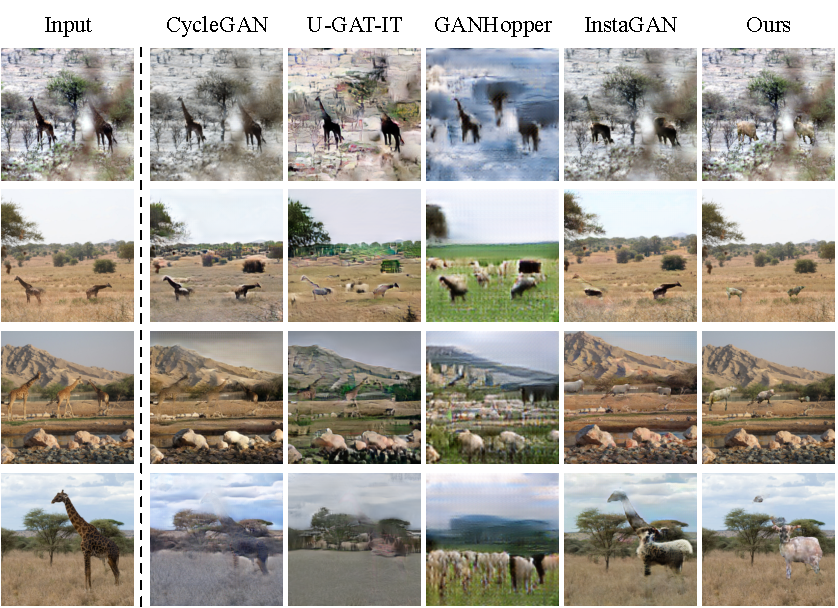
\includegraphics[width=\textwidth]{figs/gir2shp.pdf}
  \caption{长颈鹿转绵羊的定性结果图。}
  \label{fig:gir2shp}
\end{figure}

\subsubsection{客观定量评价}

绵羊转长颈鹿的定量结果和长颈鹿转绵羊的定量结果分别由表\ref{tab:shp2gir}和表\ref{tab:gir2shp}给出,FID指标评定生成图像的真实性,LPIPS指标评定生成图像的多样性。需注意的是:表中$\uparrow$代表此评价指标的值越大越好,反之$\downarrow$代表值越小越好;表中加粗的数字为最好的结果。从两个表中可以看出,GANHopper在绵羊$\leftrightarrow$长颈鹿两个任务上的FID分数都是最高的,说明它生成的结果与真实图像之间存在很大差异,这从图\ref{fig:shp2gir}和\ref{fig:gir2shp}中可以明显看出。除此之外,GANHopper在这两个任务上的LPIPS分数都是最低的,因为其生成的结果基本类似。CycleGAN在这两个任务上的FID和LPIPS指标优于GANHopper,但其生成结果还是存在一些失真,所以其FID指标在两个任务上都很低,但在长颈鹿转绵羊的任务上,结合\ref{fig:gir2shp}我们可以发现,CycleGAN并未完成翻译,生成图像和输入图像之间相差不大,所以这里LPIPS反映的是输入图像的多样性,因此分数较高。U-GAT-IT整体稍优于CycleGAN,但在两个任务上的LPIPS分数都偏低,说明其缺乏多样性。InstaGAN拥有较低的FID和较高的LPIPS分数,在绵羊转长颈鹿任务上,其FID分数与我们方法的FID分数接近,说明它真实性较好,但其LPIPS分数则显示在两个任务上与我们相差一定的多样性。本文提出的方法在绵羊转长颈鹿和长颈鹿转绵羊两个方向上都可以在获得较低FID分数的同时拥有较高的LPIPS分数,说明我们的方法生成的结果既有较高的真实性,也实现了域内的多样性,从而证明了我们方法的有效性。

\begin{table}[ht]
  \centering
  \caption{绵羊转长颈鹿的定量结果。}
    \begin{tabular}{c|c|c|c|c|c}
      \hline\noalign{\smallskip}
      方法 & CycleGAN & U-GAT-IT & GANHopper & InstaGAN & Ours \\
      \noalign{\smallskip}\hline\noalign{\smallskip}
      FID$\downarrow$   & 214.1329 & 212.0401 & 231.0558 & 192.8113 & \textbf{190.8434} \\
      LPIPS$\uparrow$ & 0.634$\pm$0.094 & 0.638$\pm$0.099 & 0.566$\pm$0.090 & 0.643$\pm$0.102 & \textbf{0.652$\pm$0.100} \\
    \noalign{\smallskip}\hline
    \end{tabular}
  \label{tab:shp2gir}
\end{table}

\begin{table}[ht]
  \centering
  \caption{长颈鹿转绵羊的定量结果。}
    \begin{tabular}{c|c|c|c|c|c}
      \hline\noalign{\smallskip}
      方法 & CycleGAN & U-GAT-IT & GANHopper & InstaGAN & Ours \\
      \noalign{\smallskip}\hline\noalign{\smallskip}
      FID$\downarrow$   & 242.0643 & 238.4553 & 276.8359 & 219.1365 & \textbf{211.4066} \\
      LPIPS$\uparrow$ & 0.662$\pm$0.100 & 0.658$\pm$0.106 & 0.608$\pm$0.103 & 0.665$\pm$0.102 & \textbf{0.673$\pm$0.102} \\
    \noalign{\smallskip}\hline
    \end{tabular}
  \label{tab:gir2shp}
\end{table}

\subsection{消融实验结果与分析}

因在多目标形变图像翻译中,形状和纹理的翻译效果对整个模型的性能起决定性作用,因此我们在形状翻译和纹理翻译阶段做消融实验。

\subsubsection{形状翻译}

为了探索不同结构的形状生成器$G_S$的作用,我们采用了三种结构组建形状生成器,第一种是下采样+上采样+跳连接,在下采样和上采样中分辨率相同的特征图之间添加跳连接,记作$G_S^{skip}$;第二种是下采样+残差块+上采样,其中残差块仅添加在下采样和上采样之间,记作$G_S^{res}$;第三种是下采样+残差块+上采样,其中残差块不仅添加在下采样与上采样之间,还添加在下采样和上采样中,共有5种尺度的残差块,记作$G_S^{multi\_res}$。

\begin{figure}[ht]
    \centering
  \includegraphics[width=.8\textwidth]{figs/ablation_study_shape.pdf}
  \caption{形状生成器采用不同结构的翻译结果示意图。}
  \label{fig:ablation_study_shape}
\end{figure}

从图\ref{fig:ablation_study_shape}可以看出,若采用$G_S^{skip}$结构,虽然会在形状上有所变化,但形状变化得不彻底,与长颈鹿的形状有一定差异,尤其是长颈鹿的头部区域,几乎没有头部的轮廓,而$G_S^{res}$可以较细致地生成长颈鹿的形状,头部和腿部生成得都较真实。这两种结构生成的图像存在差异的原因可能是在上采样过程中通过跳连接融合下采样时得到的各个尺度的特征图,使最终恢复的特征图融合了更多的低维特征,加强了输入图像对生成图像的限制能力,使生成图像不能最大限度地匹配真实样本的分布,去掉跳连接并加入残差块可解决此问题。图\ref{fig:ablation_study_shape}显示出相比较$G_S^{res}$,$G_S^{multi\_res}$可以生成更细致且逼真的结果,长颈鹿的轮廓边缘整体更流畅圆滑,且位置和身体的朝向更准确,推断产生这种结果的原因为$G_S^{res}$在单尺度上用残差块可能限制通过中间瓶颈的信息,从而限制网络的学习功能,而在上采样和下采样过程中加入残差块,使网络能够学习适用于较高和较低空间分辨率特征的多尺度转换,从而实现更彻底的形状翻译。

\subsubsection{纹理翻译}

不同结构的纹理生成器$G_T$对纹理翻译结果的影响也是我们研究的重点,纹理生成得越细致,整体图像越逼真,我们采用下采样+残差块+上采样(记作$G_T^{res}$)和下采样+上采样+跳连接(记作$G_T^{skip}$)两种结构生成纹理,除此之外,还探讨了在这两种结构的基础上加入颜色损失对纹理翻译效果的影响,分别记作$G_T^{res}$+color和$G_T^{skip}$+color。

\begin{figure}[ht]
    \centering
  \includegraphics[width=\textwidth]{figs/ablation_study_texture.pdf}
  \caption{纹理生成器采用不同结构,并分别加入颜色损失的翻译结果示意图。}
  \label{fig:ablation_study_texture}
\end{figure}

从图\ref{fig:ablation_study_texture}整体看,采用跳连接的生成效果更佳,与形状翻译不同,在此过程中,我们希望生成的纹理与输入图像所对应的纹理尽量一致,跳连接可以保证网络在翻译过程中融合并学习更多的特征信息,加入的颜色损失可进一步优化纹理的生成效果,使边缘生成得更清楚。从图\ref{fig:ablation_study_texture}可以明显看出纹理生成效果最优的为$G_T^{skip}$+color,纹理较清晰细致,且没有彩色的亮斑,因此我们的纹理生成器采用$G_T^{skip}$结构,并引入颜色损失。

\section{讨论}

从前面的实验分析中可以看出,尽管我们的方法在多目标形变图像翻译任务上可以取得比其它方法更佳的结果,但整体生成效果仍存在提升空间。目前大多数做形变翻译的工作集中于单目标形变图像翻译,输入图像无背景、目标明显,两个域的目标之间差异度较低,如狗与猫、人脸与漫画脸、人脸与猫脸等,而绵羊与长颈鹿的差异度相比较更高一些,且图像中存在多个目标,这导致多目标形变图像翻译具有极大的挑战性。我们的方法利用实例分割图获取每个目标的实例信息,并将复杂的问题分为几个小问题逐个解决,虽可以实现翻译,但当多个目标存在重叠时,目前的方法还不能实现准确地逐个翻译,所以这个问题还有待研究。

\section{本章小结}

本章介绍了多目标形变图像翻译问题,并为解决此问题提出我们基于生成对抗网络的模型。

在第一节中,我们简要介绍了形变翻译与侧重纹理翻译任务的区别,并进一步介绍了多目标形变图像翻译任务。

在第二节中,我们确定了多目标形变图像翻译需要考虑两个问题,且在探索过程中发现实例分割图更易于完成形状翻译,因此提出了一个模型,将形状、纹理和背景分开处理,融合细化后得到最终的生成图像,还介绍了各部分的网络结构及其对应的目标函数。

在第三节中,我们介绍了实验用到的数据集、对比方法和评价指标,并从定性和定量两方面分析实验结果,对形状翻译和纹理翻译部分的生成器结构和损失做了相应的消融实验,从实验显示的结果确定最优的方案。

在最后一节中,我们讨论了本方法存在的一些局限性,并指出需要改进的地方,确定了今后的研究方向。

